\documentclass[xetex,mathserif,serif]{beamer}
\usepackage{polyglossia}
\setdefaultlanguage[babelshorthands=true]{russian}
\usepackage{minted}
\usepackage{tabu}
\usepackage{pgfplots}
\usepackage{textpos}

\useoutertheme{infolines}

\usepackage{fontspec}
\setmainfont{FreeSans}
\newfontfamily{\russianfonttt}{FreeSans}

\usepackage{forest}
\usetikzlibrary{arrows}

\setbeamertemplate{blocks}[rounded][shadow=false]
\setbeamercolor*{block title example}{fg=green!50!black,bg=green!20}
\setbeamercolor*{block body example}{fg=black,bg=green!10}

\setbeamercolor*{block title alerted}{fg=red!50!black,bg=red!20}
\setbeamercolor*{block body alerted}{fg=black,bg=red!10}

\tabulinesep=0.7mm

\title{``Динамические'' структуры данных}
\subtitle{Что ещё можно делать с указателями}
\author[Юрий Литвинов]{Юрий Литвинов \newline \textcolor{gray}{\small\texttt{y.litvinov@spbu.ru}}}

\date{12.10.2021}

\begin{document}
	
	\frame{\titlepage}
	
	\begin{frame}[fragile]
		\frametitle{Структуры, ссылающиеся сами на себя}
		\begin{footnotesize}
			\begin{minted}{cpp}
typedef struct Element {
    int value;
    struct Element* next;
} Element;

void main() {
    Element* element1 = malloc(sizeof(Element));
    Element* element2 = malloc(sizeof(Element));
    element1->next = element2;
    free(element1);
    free(element2);
}
			\end{minted}
		\end{footnotesize}
	\end{frame}

	\begin{frame}
		\frametitle{Стек на указателях}
		Структура данных, в которой элемент можно добавлять только в начало и забирать только из начала (LIFO, Last In --- First Out)
		\begin{columns}
			\begin{small}
				\begin{column}{0.55\textwidth}
					\begin{itemize}
						\item Может хранить ``сколько угодно'' данных
						\begin{itemize}
							\begin{scriptsize}
							\item Можно сделать стек ещё на массивах, но тогда он будет ограничен по размеру
							\end{scriptsize}
						\end{itemize}
					\end{itemize}
				\end{column}
			\end{small}
				\begin{column}{0.45\textwidth}
					\begin{center}
						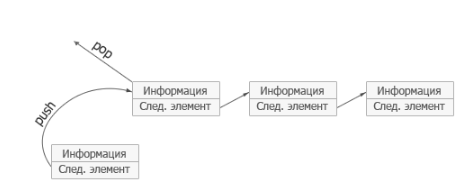
\includegraphics[width=0.95\textwidth]{stack.png}
					\end{center}
				\end{column}
		\end{columns}
		\begin{itemize}
		\item Используется везде
			\begin{itemize}
				\begin{scriptsize}
				\item Для организации рекурсии
				\item Для синтаксического анализа программ
				\item Для проверки корректности скобок
				\item Для арифметических вычислений
				\item Для исполнения программ (.NET --- пример стековой машины)
				\item ...
				\end{scriptsize}
			\end{itemize}
		\end{itemize}
	\end{frame}

	\begin{frame}
		\frametitle{Очередь}
		Структура данных, в которой элемент можно добавлять только в конец и забирать только из начала (FIFO, First In --- First Out)
		\begin{columns}
			\begin{column}{0.6\textwidth}
				\begin{itemize}
					\item Используется для
					\begin{itemize}
						\item Обмена сообщениями между параллельными потоками
						\item Обработки событий от пользователя или от операционной системы
						\item ...
					\end{itemize}
				\end{itemize}
			\end{column}
			\begin{column}{0.4\textwidth}
				\begin{center}
					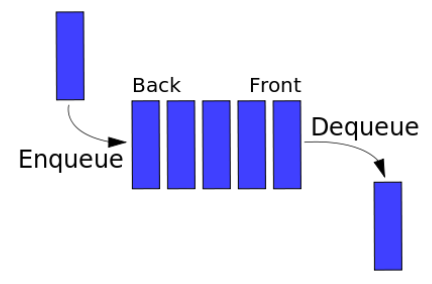
\includegraphics[width=0.9\textwidth]{queue.png}
				\end{center}
			\end{column}
		\end{columns}
	\end{frame}

\end{document}